\chapter{Radial Basis Function}

\section{Least Square Estimator}
Linear Regression Equations:
\begin{equation*}
\begin{split}
y &= \sum_{i=1}^{n} w_i f_i(\mathbf{x}) \\
&= w_1 f_1(\mathbf{x}) + w_2 f_2(\mathbf{x}) + \ldots + w_n f_n(\mathbf{x})  \\
\mathbf{y} &= \mathbf{Aw}
\end{split}
\end{equation*}
The squared error:
\begin{equation*}
\begin{split}
E &=\| \mathbf{y -d} \|^{2} \\
&= \| \mathbf{d - Aw} \|^{2} \\
&= \mathbf{(d-Aw)^{T}(d-Aw)} \\
&= \mathbf{d^{T}d - d^{T}Aw - (Aw)^{T}d + (Aw)^{T}(Aw)} \\
&= \mathbf{d^{T}d - 2w^{T}A^{T}d + w^{T}A^{T}Aw}
\end{split}
\end{equation*}
For least-square estimator:
\begin{equation*}
\begin{split}
\frac{\partial E}{\partial \mathbf{w}} &= 0 \\
2\mathbf{A^{T}d} - 2\mathbf{A^{T}Aw} &= 0 \\
\mathbf{A^{T}Aw} &= \mathbf{A^{T}d} \\
\mathbf{w} &= \mathbf{(A^{T}A)^{-1}A^{T}d}
\end{split}
\end{equation*}
If A is non-singular, $\mathbf{(A^{T}A)^{-1}A^{T}}$ is pseudoinverse of A. \\
If A is singular, pseudoinverse is same as inverse of matrix. \\
Singular matrix: Square matrix that is not invertible.

\section{Cover's Separability Theorem}
A complex pattern-classification problem cast in a high-dimensional hidden space non-linearly is more likely to be linearly separable than in a low-dimensional input space.

\section{Basis Function Network}
\begin{figure}[h]
\centering
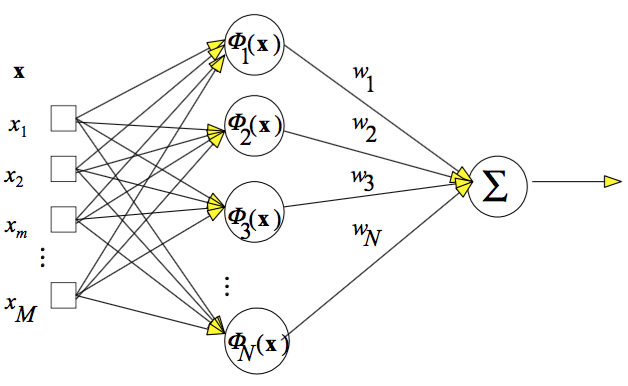
\includegraphics[width=10cm]{chapter5_1}
\end{figure}
$$f(\mathbf{x}) = y = \sum_{i=1}^{N} w_i \phi_i(\mathbf{x})$$
The radial basis functions technique consists of choosing a basis function of the following form:
$$f(\mathbf{x}) = \sum_{i=1}^{N} w_i \phi(\| \mathbf{\mathbf{x-\mu_{i}}}\|)$$

\section{Typical Radial Basis Functions}
Piecewise linear approximation:
$$\phi(\| \mathbf{x} - \pmb{\mu_{i}}\|) = \| \mathbf{x} - \pmb{\mu_{i}} \|$$
Cubic approximation:
$$\phi(\| \mathbf{x} - \pmb{\mu_{i}}\|) = \| \mathbf{x} - \pmb{\mu_{i}} \|^{3}$$
Gaussian function:
$$\phi(\| \mathbf{x} - \pmb{\mu_{i}}\|) = exp(-\frac{\| \mathbf{x} - \pmb{\mu_{i}} \|^{2}}{2 \sigma^{2}})$$
Thin plate splines:
$$\phi(\| \mathbf{x} - \pmb{\mu_{i}}\|) = \| \mathbf{x} - \pmb{\mu_{i}} \|^{2} log(\| \mathbf{x} - \pmb{\mu_{i}} \|)$$
Multiquadratic function:
$$\phi(\| \mathbf{x} - \pmb{\mu_{i}}\|) = (\| \mathbf{x} - \pmb{\mu_{i}} \|^{2} + \sigma^{2})^{1/2}$$
Inverse multiquadratic function:
$$\phi(\| \mathbf{x} - \pmb{\mu_{i}}\|) = (\| \mathbf{x} - \pmb{\mu_{i}} \|^{2} + \sigma^{2})^{-1/2}$$

\section{RBF as Interpolation Networks}
In the interpolation approach,RBF technique consists of choosing a function such that:
\begin{equation}
f(\mathbf{x}) = y = \sum_{i=1}^{L} w_i \phi(\| \mathbf{x - x_{i}} \|^{2})
\label{interpolation}
\end{equation}
And the interpolation condition is:
\begin{equation}
f(\mathbf{x}) = \mathbf{d}
\label{interpolation_condition}
\end{equation}
Let:
\begin{equation}
\phi_{li} = \phi(\| \mathbf{x_l - x_i} \|)
\label{temp4}
\end{equation}
Substituting \ref{interpolation_condition} and \ref{temp4} to \ref{interpolation}
\begin{equation}
\begin{split}
\sum_{i=1}^{L} w_i \phi(\| \mathbf{x_l - x_{i}} \|^{2}) &= d_l \\
\sum_{i=1}^{L} w_i \phi_{li} &= d_l
\end{split}
\end{equation}
Rewrite the equation in matrix form:
$$
\begin{bmatrix}
\phi_{11}  & \cdots & \phi_{1N} \\
\vdots     & \ddots & \vdots \\
\phi_{N1}  & \cdots & \phi_{NN}   
\end{bmatrix}
\begin{bmatrix}
w_1 \\
\vdots \\
w_N
\end{bmatrix} = 
\begin{bmatrix}
d_1 \\
\vdots \\
d_N
\end{bmatrix}
$$
$$\pmb{\phi w = d}$$
Assuming \emph{Gram Matrix} $\phi$ is non-singular:
$$\pmb{w = \phi^{-1} d}$$
\textit{Note: The number of hidden nodes is equal to the number of data points}

\section{RBF as Approximation Networks}
In a generalized Gaussian RBF network, each hidden node represents a cluster of patterns. 
\begin{equation}
\begin{split}
\phi(\| \mathbf{x} - \pmb{\mu_{i}}\|) &= exp\Big(-\frac{\| \mathbf{x} - \pmb{\mu_{i}} \|^{2}}{2 \sigma^{2}} \Big) \\
&= exp\Big(- \frac{1}{2} (\mathbf{x} - \pmb{\mu_i})^{T} \mathbf{C_i^{-1}} (\mathbf{x} - \pmb{\mu_i}) \Big)
\end{split}
\end{equation}
The centroid $\pmb{\mu}$ and covariance matrix $\mathbf{C}$: 
$$\pmb{\mu_{i}} = \frac{1}{L} \sum_{j=1}^{L} \mathbf{x_j}$$
$$\mathbf{C_i} = \frac{1}{L-1} \sum_{j=1}^{L} (\mathbf{x_j} - \pmb{\mu_i})(\mathbf{x_j} - \pmb{\mu_i})^{T}$$
RBF use k-means clustering algorithm to learn centroids of hidden layer neurons. 